%!LW recipe=pdflatex-shellescape
\documentclass[11pt]{article}

\usepackage[margin=1.25in, top=1in, bottom=1in]{geometry}

\usepackage[utf8]{inputenc}
%\usepackage[english]{babel}

\usepackage{graphicx}
\usepackage[dvipsnames,svgnames]{xcolor}
\usepackage{amsmath}
\usepackage{float}
\usepackage{natbib}
\bibliographystyle{mnras}
\setcitestyle{authoryear,open={(},close={)}}
%\usepackage[hybrid]{markdown}
\usepackage{enumitem}
\setitemize{itemsep=-2pt}
\usepackage[colorlinks=true,allcolors=blue]{hyperref}
\usepackage{caption}
\usepackage{overpic}
\usepackage{amssymb}
\usepackage{multirow}
\usepackage{mathtools} 
\usepackage{lipsum}
\usepackage{fancyheadings}
\usepackage{tcolorbox}
\usepackage{listings}
\usepackage{fancyvrb}         % better verbatim support
\usepackage{etoolbox} % for patching
\usepackage{pagecolor}
\usepackage{pgffor} % for "for" loops

\usepackage{showlabels}
% ========== layout for the marginal notes ==========
\renewcommand{\showlabelsetlabel}[1]{
  \hspace{-15pt}
  \parbox[t]{1.25in}{\raggedright\footnotesize\color{gray}#1}%
}
            
\renewcommand{\subsectionmark}[1]{%
  \markright{\MakeUppercase{\thesubsection.\ #1}}}%

\pagestyle{fancy}
\fancyhead[L]{}
\fancyhead[R]{\nouppercase{\rightmark}}
\fancyfoot[R]{\vspace{-5pt}\rule{\textwidth}{0.4pt}\\ \thepage}
\fancyfoot[C]{\protect\color{gray}\today}

\tcbset{textmarker/.style={%
        parbox=false,boxrule=0mm,boxsep=0mm,arc=0mm,
        outer arc=0mm,left=2mm,right=2mm,top=7pt,bottom=7pt,
        toptitle=1mm,bottomtitle=1mm,oversize}}
        
% define new colorboxes
% add breakable ?
\newtcolorbox[auto counter,number within=chapter]{hintBox}[1][]{textmarker, colback=yellow!10!white}
\newtcolorbox{importantBox}{textmarker, colback=red!10!white}
\newtcolorbox{noteBox}{textmarker, colback=green!10!white}

% define commands for easy access
\newcommand{\note}[2]{\begin{noteBox} \textbf{#1} #2 \end{noteBox}}
\newcommand{\warning}[2]{\begin{hintBox} \textbf{#1} #2 \end{hintBox}}
\newcommand{\important}[2]{\begin{importantBox} \textbf{#1} #2 \end{importantBox}}

% Patch \section to prevent it from writing into ToC automatically
\makeatletter
\pretocmd{\@sect}{\if@toccoloring\else}{}{}
\apptocmd{\@sect}{\fi}{}{}
\newif\if@toccoloring
\makeatother

\newcommand{\coloredsection}[2]{%
  \refstepcounter{section}% increase the section counter
  \section*{\color{red}\thesection\quad #2}% print number + title manually
  \addcontentsline{toc}{section}{\textcolor{#1}{\thesection\quad #2}}%
}

\newcommand{\coloredsubsection}[2]{%
  \refstepcounter{subsection}% increase the section counter
  \subsection*{\color{red}\thesubsection\quad #2}% print number + title manually
  \addcontentsline{toc}{subsection}{\textcolor{#1}{\thesubsection\quad #2}}%
}

\newcommand{\coloredsubsubsection}[2]{%
  \refstepcounter{subsubsection}% increase the section counter
  \subsubsection*{\color{red}\thesubsubsection\quad #2}% print number + title manually
  \addcontentsline{toc}{subsubsection}{\textcolor{#1}{\thesubsubsection\quad #2}}%
}

\definecolor{lightred}{RGB}{255, 245, 245}

\newcommand{\includeOrGrayBox}[1]{%
  \IfFileExists{#1}{%
    \includegraphics[width=0.09\textwidth]{#1}%
  }{%
    \textcolor{lightgray}{\rule{0.09\textwidth}{0.09\textwidth}}
  }%
}

\title{\vspace{10em} \Huge Topology Project:\\ Research Notes\vspace{2em}}

\author{\LARGE Alexandre Champagne-Ruel\vspace*{1em}}

\begin{document}

\maketitle
\clearpage

\tableofcontents
\clearpage

\section{Previous notes from Cole}
\label{sec:previous-notes}

\subsection{May 12th, 2022}

I'm starting a notebook because I keep forgetting what I'm working on. Hopefully this will complement the git logs.

Today I was able to update the \texttt{Ensemble} constructor function and write a function in \texttt{explore-parameters.jl} that will generate an Ensemble and run the dynamics. I need to check for bugs and work on the visualization side now.

I need to make sure to use \texttt{@quickactivate} with DrWatson; otherwise, saving does not work as expected.

\subsection{June 24th, 2022}

I should focus on this project a bit more. My goal today is to make a plan of attack. This should include a few different things, mostly issues on git to guide future development.\\

\textbf{Main goals:}

\begin{itemize}
    \item Parameter sweep of the well-mixed case:
    \begin{itemize}
        \item Plot Max MA, MA distribution fit, integer number against (forward, backward rate)
    \end{itemize}

    \item Parameter sweep of spatially distributed cases:
    \begin{itemize}
        \item Plot same things against diffusion rates
        \item Start with Line Graphs, then lattice, then random.
        \item Compute MA of Graphs. (Pick forward/backward rate from sweep above and vary diffusion)
    \end{itemize}
\end{itemize}

To do those we'll need a coherent data management system and an efficient analysis pipeline.

\subsection{July 6th, 2022}

Taking a look after a couple of days away. The Simulation class is implemented now. I think the main thing to do is convert the .bson files to a .csv (somewhat efficiently) and then write some R scripts to do the analysis we want.

The save system is working; now it's time to write the analysis pipeline.

\subsection{July 12th, 2022}

Analysis pipeline mostly sorted out. There's likely some bugs lurking about, and I don't know what will happen at scale, but we'll see. The big problem now is mostly a problem for the future: once specific compounds are stabilized by different reactors, it will be difficult to keep track of all the information in coherent ways. The same problem exists for simulations with different rate constants in different reactors.

Need to check the assumptions of the simulation.

\subsection{July 13th, 2022}

Lots of systems in place now. Just debugging the simulations before running the parameter sweep. Something disturbing is the degree to which the reactors without inflow seem to be completely static for all time. This strikes me as a serious bug. I can't seem to find the source.

\subsection{September 9th, 2024 (Alex)}

\begin{itemize}
    \item Seems like Cole has fixed the function call in \texttt{test\_timing.jl}. I have launched several simulations varying the parameter set, and it executes normally.
    \item I am now trying to get the parameter explorations to work (\texttt{test\_timing.jl} and \texttt{explore-test.jl}), ideally using multiple CPU cores. The original file coded by Cole (\texttt{explore-test.jl}) was still looping sequentially over the different parameters, which is why I have made a new version (\texttt{explore-test.jl}) that computes the different parameter permutations in advance and launches the simulations using these pre-computed parameters. It seems to use the full extent of the multiprocessing module, as observed from CPU usage in e.g., \texttt{htop}.
\end{itemize}

\subsection{September 11th, 2024  (Alex)}

\begin{itemize}
    \item Did a bunch of tests in the past few days—\texttt{test\_timing.jl} and \texttt{explore-test.jl} are now working on Sol, the GCloud cluster, etc.
\end{itemize}

\subsection{September 12th, 2024  (Alex)}

\begin{itemize}
    \item Started coding a minimal working example: plotting the population time series.
\end{itemize}

\clearpage

\section{Description of the system}
\label{sec:desc-system}

\subsection{Artificial chemistry}
\label{subsec:artificial-chemistry}

Basically, we want to use a system based on artificial chemistry to investigate the conditions promoting the formation of complex objects---where, by "complex objects", we refer to molecular complexity. Specifically, we will be focusing our analysis on investigating the spatial topology of the environment, to try to determine how it can program the emergence of complexity. We will utilize Assembly Theory to quantify the complexity formed therein, and in doing so this model will constitute a new test environment. Among other things, this could help refine our methods of calculation for the Assembly Index, and inform our knowledge on how the Assembly Index responds to various parameters and/or is correlated to life-like properties.

Artificial chemistry implementations can be categorized along two axis: how abstract (or realistic) they represent "real" chemistry, and whether they aim to model early or late evolution (see~Fig.~\ref{fig:abstraction-stage}).

\begin{figure}[hbt]
  \centering
  {\LARGE Approaches to artificial chemistry}\vspace{1em}\\
  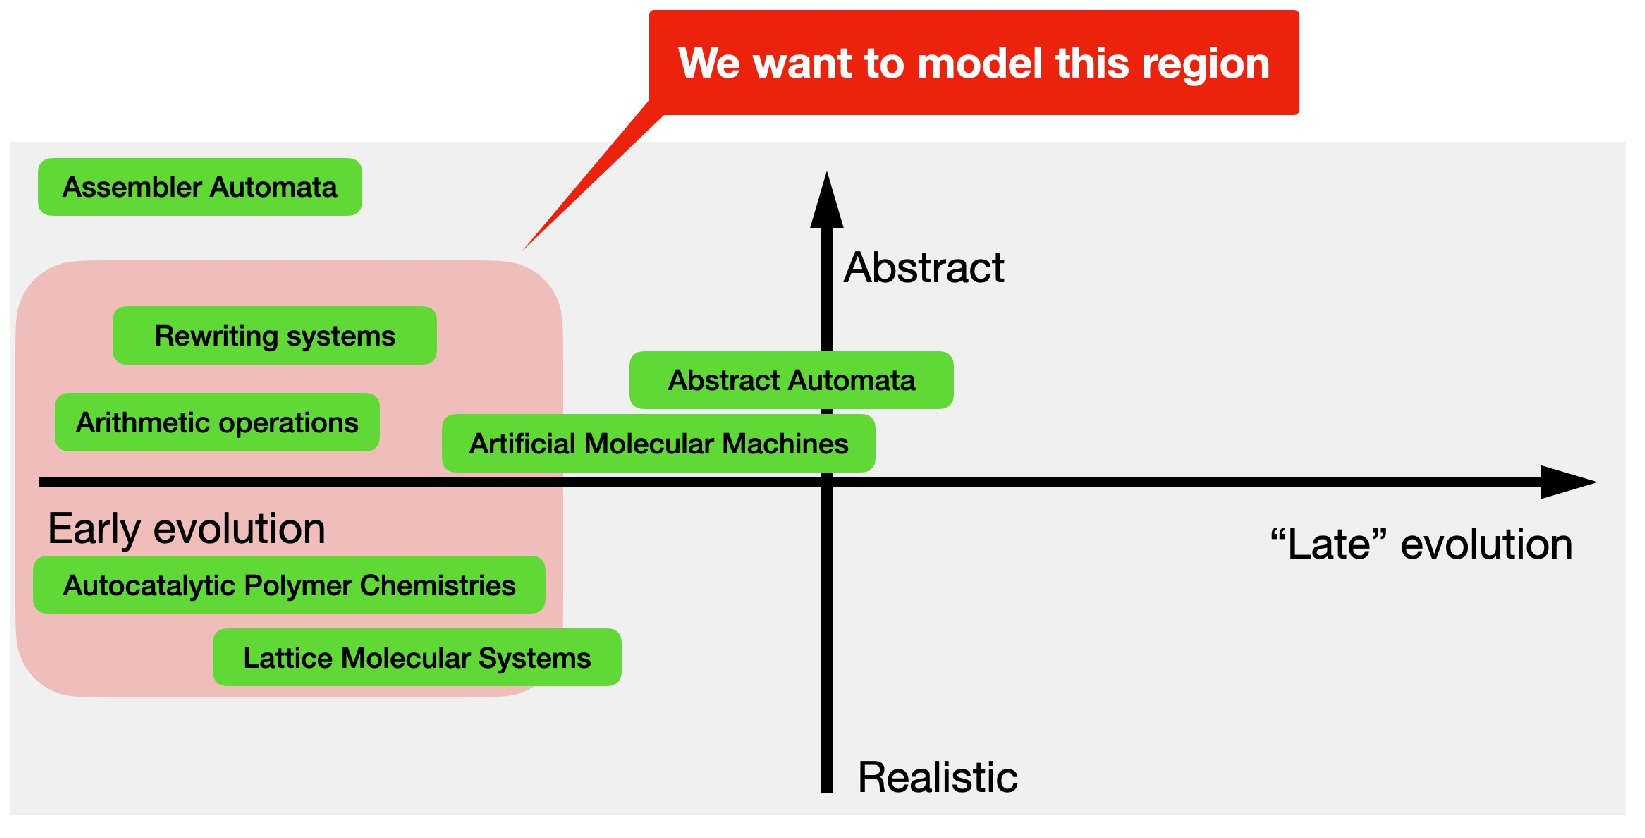
\includegraphics[width=0.90\textwidth]{figures/system/abstraction-stage.pdf}
  \caption{Classification of AC approaches along two axis: abstract vs realistic, and early vs late evolution. In the context of this project we will be focusing on the early evolution, using a balanced approach between more abstract and more realistic models.}
  \label{fig:abstraction-stage}
\end{figure}

The underlying (artificial) chemistry is based on several transformations: formard reactions, backward reactions, diffusion (Table~\ref{tab:reactions}). These reactions are parametrized by rate coefficients ($k_f$, $k_b$, $k_d$). Several other parameters can be defined, such as simulations (temporal) length $\tau_{max}$, the number of reactors $N$, the number of inflows $n$, total mass $M$, etc.\\

\begin{table}[h]
\centering
\begin{tabular}{|c|c|}
\hline Forward reaction & $A+B \xrightarrow{k_f} C$ \\
\hline Backward reaction & $C \xrightarrow{k_b} A^{\prime}+B$ \\
\hline \multirow{2}{*}{ Diffusion } & $C \xrightarrow{k_d} \varnothing$ \\
\cline { 2 - 2 } & $C_i \xleftrightarrow{k_d} C_j$ \\
\hline
\end{tabular}  
\caption{Reactions occurring in the artificial chemistry implemented in this system. Forward (constructive) reactions happens at rate $k_f$, backward (destructive) reactions happen at rate $k_b$ and diffusion (where a molecule is shifted either to the next chemostat or out of the system) happens at rate $k_d$. Mass $M$ is fixed, so the in-flow is coupled with the diffusion parameter.}
\label{tab:reactions}
\end{table}

\note{Backward Reaction Rate.}{We have chosen to keep the backward reaction rate \textit{constant} with respect to molecule length (i.e., integer value). Both alternatives can be justified: larger molecules might break more easily due to having more bonds, or they might be harder to break because they are more stable. Here, we adopt the former assumption.}

\subsection{System of reactors}
\label{subsec:system-of-reactors}

These transformations are applied on a population of integers. These integers form a well-mixed system, inside a reactor/chemostat (Fig.~\ref{fig:reactor-ensemble}a). The number of integers \#1 is fixed, which translates into a fixed in-flow in the first reactor (as these integers are used to form other, more complex integers, or diffuse to the next chemostats). The system as a whole consists of several of these reactors, coupled together via in- and out-flows (defined by the corresponding rates), in a specific topology. For example, one of the simplest topology is that of the regular lattice (Fig.~\ref{fig:reactor-ensemble}b). When diffusion is very high, the whole system becomes well-mixed.

\begin{figure}[hbt]
  \centering
    {\LARGE Diagram of reactor + ensemble of reactors}\vspace{1em}\\
  \begin{overpic}[width=0.35\textwidth]{figures/system/single-reactor.pdf}\put(-15,85){\textbf{(A)}}\end{overpic}\hspace{0.10\textwidth}
  \begin{overpic}[width=0.40\textwidth]{figures/system/ensemble.pdf}\put(-15,95){\textbf{(B)}}\end{overpic}
  \caption{\textbf{(A)} Single reactor, inside of which a bunch of integers react. In-flow is fixed, i.e. the \# of ones is fixed, and these react according to the reactions described in Table~\ref{tab:reactions}. An out-flow connects the reactor to subsequent chemostats. \textbf{(B)} Network of reactors/chemostats. Displayed is a regular lattice (note that diffusion happens both ways). There is a single in-flow, and a single out-flow. Other topologies are possible (see Fig.~\ref{fig:topologies} below.)}
  \label{fig:reactor-ensemble}
\end{figure}

\subsection{Topologies}
\label{subsec:topologies}

Several topologies can be used to connect the reactors together (Fig.~\ref{fig:topologies}). Examples include: path, lattice, Erdos-Renyi (random), regular (uniform node degree) or Barabasi-Albert (power-law degree distribution). This is especially relevant given that we’re studying living systems, whose networks have been shown to possess certain specific properties deriving from their topology (e.g., resilience from BA networks, etc.) Other topologies (e.g. lattice, random) can be used as control/neutral.

\begin{figure}[hbt]
  \centering
    {\LARGE Examples of topologies}\vspace{1em}\\
  \begin{overpic}[width=0.05\textwidth]{figures/system/graph-path.pdf}\put(-15,95){\textbf{(A)}}\end{overpic}
  \hspace{0.30\textwidth}
  \begin{overpic}[width=0.20\textwidth]{figures/system/graph-lattice.pdf}\put(-15,100){\textbf{(B)}}\end{overpic}\\
  \begin{overpic}[width=0.25\textwidth]{figures/system/graph-ER.pdf}\put(-5,80){\textbf{(C)}}\end{overpic}
  \hspace{0.05\textwidth}
  \begin{overpic}[width=0.25\textwidth]{figures/system/graph-regular.pdf}\put(-15,80){\textbf{(D)}}\end{overpic}
  \hspace{0.05\textwidth}
  \begin{overpic}[width=0.25\textwidth]{figures/system/graph-BA.pdf}\put(-5,80){\textbf{(E)}}\end{overpic}
  \caption{Illustrations of the different topologies we’ll be exploring (at least, in the near future). The chemostats can be connected according to any of these topologies, which we presume will affect the construction of molecular complexity in the mixture. \textbf{(A)} Simple path lattice. \textbf{(B)} Lattice. \textbf{(C)} Random (Erdos-Rényi) graph. \textbf{(D)} Regular graph (all nodes have the same degree). \textbf{(E)} Scale-free (Barabasi-Albert) graph, with the distribution of nodes follow a power law.}
  \label{fig:topologies}
\end{figure}

\subsection{Integer chemistry and Assembly Theory}
\label{subsec:integer-chemistry}

We’ll be using Assembly Theory to quantify the complexity emerging from the mixture, therefore we’ll use the Assembly Index ($A$). Cole has calculated $A$ for integers $<10000$. The Assembly Index increases as the logarithm of integer values (Fig.~\ref{fig:integers-assembly}). We’ll however probably be using both, as some relationships are better illustrated using y-axis as integers, and others with the y-axis as the Assembly Index.

\begin{figure}[hbt]
  \centering
  {\LARGE Relationship integers vs. assembly index}\vspace{1em}\\
  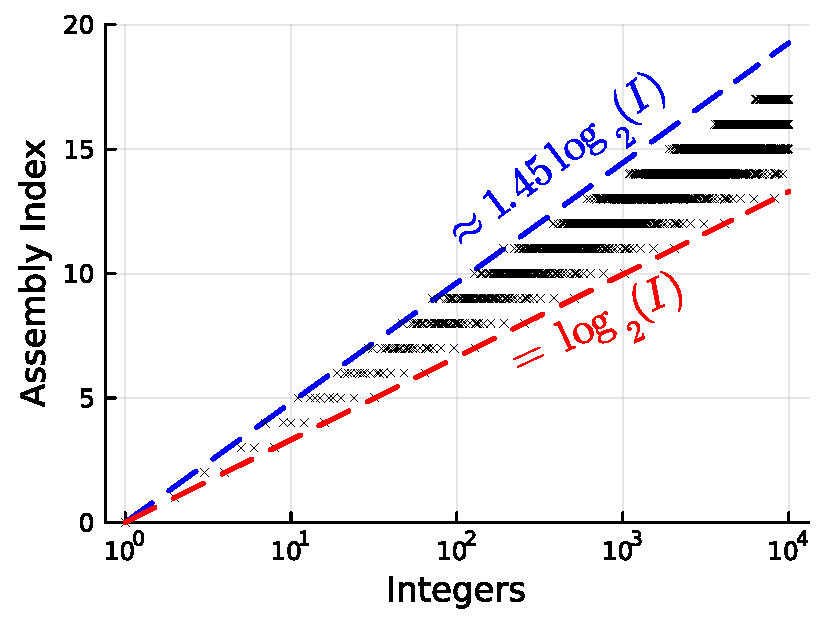
\includegraphics[width=0.40\textwidth]{figures/system/integers-assembly.pdf}
  \caption{Assembly Index $A$ for integers $<10000$. $A$ increases as the logarithm of integer values.}
  \label{fig:integers-assembly}
\end{figure}

\clearpage

\section{Experiments with the stochastic method}
\label{sec:experiments}

\subsection{MS01: time series}
\label{subsec:MS01}

A first result we can plot using this system is the time series of the populations (shown on Fig.~\ref{fig:time-series}). The layout of this figure follows the same structure as the one on Fig.~\ref{fig:reactor-ensemble}b: each panel shows the evolution of integers $I\in{1...10}$ through time. The blue curve shows ones, we can see the number of ones is fixed on the first panel (top left). Diffusion pushes molecules to the next chemostats that are connected to the first one (where the in-flow is) so we’re seeing initial transients/peaks at different times. The higher we increase diffusion, the faster these peaks happen, and the shorter is the initial transient.

\begin{figure}[hbt]
  \centering
  {\LARGE Example of time series for an ensemble of reactors}\vspace{1em}\\
  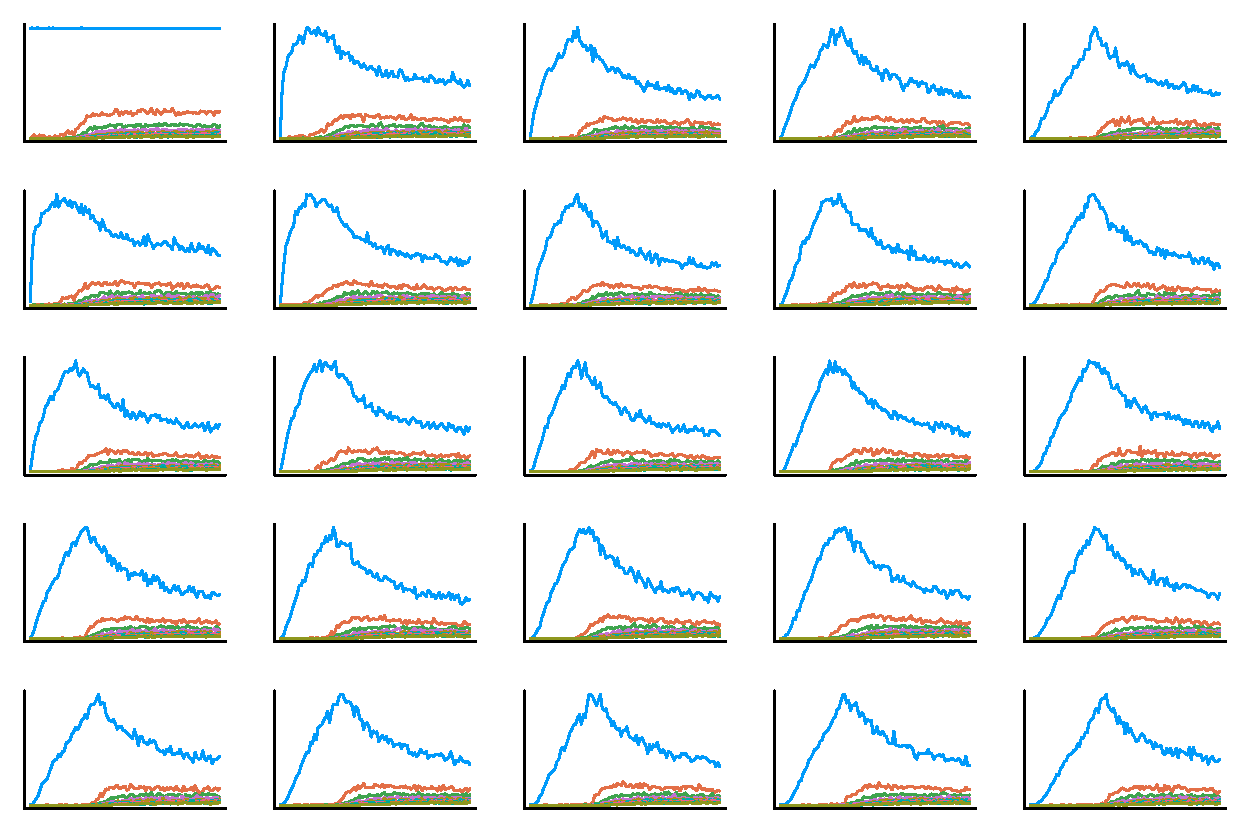
\includegraphics[width=0.75\textwidth]{figures/results/1-prelim/ts-gridplot.pdf}
  \caption{Time series for a simulation of 25 chemostats connected in a regular lattice. The first panel (top left) corresponds to the chemostat with an in-flow connected to it. The ten first species (integers $I\in{1...10}$) are shown.}
  \label{fig:time-series}
\end{figure}

\clearpage

\subsection{MS02: varying the diffusion rate}
\label{subsec:MS02}

A first parameter we’re exploring is the diffusion rate. We’ve sampled simulations with diffusion rates $k_d\in[10^{-6},10^{2}$ and plot the first ten species (excluding ones) on Fig.~\ref{fig:prelim-abundance}. Panel A shows the average populations across reactors, i.e. taking all the chemostats together as one single population and calculating the average for species $S$ at the last iteration of the simulation $\tau_{max}$. We’ve done this calculation for 100 values of $k_d$ (without using statistical ensembles for now). The shaded area on Panel A represents the standard deviation across chemostats, and is also illustrated on Panel B. We’ve also added a vertical (dashed) line to indicade the forward rate $k_f$. 

One thing we can readily notice from Fig.~\ref{fig:prelim-diffusion} is the presence of transitions. On Panel A we have four regimes: low values in the populations of complex (i.e. $I>1$) species for lower values of the diffusion coefficient ($k_d < k_f$), then increasing complexity ($k_f < k_d < 1$), then a dip in complexity ($k_d ~ 10$), and finally complexity increasing again for very high diffusion rates ($k_d \gtrsim 10^2$). Panel B shows an increase in $\sigma$ until $k_d ~ 10^{-1}$ then a sharp decrease ($10^{-1} < k_d < 10$).

\begin{figure}[hbt]
  \vspace{2em}
  \centering
  {\LARGE Populations (and their std) across diffusion rates}\vspace{3em}\\
  \begin{overpic}[width=0.45\textwidth]{figures/results/1-prelim/mu-vs-kd.pdf}\put(-5,80){\textbf{(A)}}\end{overpic}
  \begin{overpic}[width=0.45\textwidth]{figures/results/1-prelim/sd-vs-kd.pdf}\put(-5,80){\textbf{(B)}}\end{overpic}
  \caption{\textbf{(A)} Average populations, calculated across all chemostats, at $\tau_{max}$ for the first ten integers excluding ones. Shaded area represents the standard deviation (also pictured on Panel B). \textbf{(B)} Standard deviation for the same species shown on Panel A.}
  \label{fig:prelim-diffusion}
\end{figure}

Another thing we can calculate from these systems is the total mass, i.e. $I_i \times f_i$ (where $I_i$ is the integer of species $i$ and $f_i$ the number of identical copies or "copy number"). Shown on Fig.~\ref{fig:prelim-diffusion} is the total mass $M$ against the same variation in coefficient discussed above. $M$ stays constant for most values of the diffusion coefficient but increases exponentially for the highest values of $k_d$.\\

\begin{figure}[hbt]
  \centering
  {\LARGE Total mass of the system vs diffusion coefficient}\vspace{1em}\\
  \begin{overpic}[width=0.45\textwidth]{figures/results/1-prelim/mass.pdf}\end{overpic} \\
  \caption{Increase in total mass as we increase diffusion. Total mass $M$ is calculated by multiplying integers $I_i$ with their copy number $f_i$.}
  \label{fig:prelim-mass}
\end{figure}

\note{Putting this all together:}{There seems to be three regimes based on what we’re seeng in Figs~\ref{fig:prelim-diffusion}-\ref{fig:prelim-mass}: initially, we have a well-mixed system in the first chemostat. The complexity in chemostat \#1 increases, but all other chemostats remain empty, which is why we’re seeing low average values in Fig.~\ref{fig:prelim-diffusion} (they’re calculated over all chemostats). Then, as we increase diffusion the other chemostats are progressively filled up: this is why the standard deviation increases. Finally, as all chemostats are fully filled and we continue increasing the diffusion, the system returns to a well-mixed state and the mass increases rapidly (because complexity now builds up in all the chemostats).}

\clearpage

\subsection{MS03: measuring distance from source}
\label{subsec:MS03}

One additional experiment we’ve done was to investigate how the mean assembly index (per reactor) varied with the distance from source $D$. For example, the distance $D$ between the source (in green) and the target chemostat (in red) shown on Fig.~\ref{fig:prelim-distance}a would be six. We’ve evaluated how the complexity varied with $D$ for three diffusion regimes: low diffusion ($k_d=10^{-4}$), intermediate diffusion ($k_d = 10^{-2}$) and high diffusion ($k_d=10$). Complex molecules remain in the chemostats that are located close to the source $D=1,2$ when diffusion is low (Fig.~\ref{fig:prelim-distance}, blue curve) or intermediary (red curve). When diffusion is increased (green curve), complexity spreads to the other reactors.

However, there remains a degeneracy when we examine the complexity contained in chemostats located at identical distances from the source (Fig.~\ref{fig:prelim-distance}, dashed box surrounding data points at $D=5$). Multiple chemostats at $D=5$ have different (average values of the) assembly index. This is clearly evident when looking at the inset in Fig.~\ref{fig:prelim-distance} that displays the density plots (i.e., reconstructed PDF): the heavy tails extending to high values of $A$ clearly differ from one chemostat to another. Consequently, $D$ alone does not fully determine the quantitative complexity of the mixture.

\begin{figure}[hbt]
  \centering
  \hspace{2em}
  {\LARGE Mean assembly index vs distance from the source}\vspace{1em}\\
  \begin{overpic}[width=0.33\textwidth]{figures/results/1-prelim/ensemble-distance.pdf}\put(-15,80){\textbf{(A)}}\end{overpic}
  \hspace{0.10\textwidth}
  \begin{overpic}[width=0.40\textwidth]{figures/results/1-prelim/AI-vs-D.pdf}\put(-5,70){\textbf{(B)}}\end{overpic}
  \caption{\textbf{(A)} Here we investigate how complexity varies as a function of the distance $D$ from the source. For example, the distance between the in-flow (green) and the target chemostat (red) is six. \textbf{(B)} Complexity as a function of the distance from the source, for three diffusion regimes. Inset: density plots for the four chemostats having $D=5$. Clearly, $D$ alone does not fully determine the complexity of the mixture.}
  \label{fig:prelim-distance}
\end{figure}

\clearpage

\subsection{MS04: measuring detection thresholds}
\label{subsec:MS04}

Next, we want to relate these experiments to observational missions by evaluating thresholds in complexity that we could detect. We can therefore evaluate the abundance of the different species (i.e., populations as a fraction of total \# of molecules or total mass---here we chose the former) and determine the most complex molecule we could detect using an instrument capable of measuring concentrations of $10^{-5}$ (i.e. 1 molecule in a system having a total of $10^5$ molecules), then $10^{-4}$, and so on. Fig.~\ref{fig:prelim-abundance} how the complexity of detectable molecules varies as we change the diffusion coefficient.

\begin{figure}[hbt]
  \centering
  {\LARGE Detection thresholds vs diffusion coefficient}\vspace{1em}\\
  \begin{overpic}[width=0.40\textwidth]{figures/results/1-prelim/abundance-I.pdf}\put(-5,70){\textbf{(A)}}\end{overpic}
  \hspace{0.05\textwidth}
  \begin{overpic}[width=0.40\textwidth]{figures/results/1-prelim/abundance-A.pdf}\put(-5,70){\textbf{(B)}}\end{overpic}
  \caption{\textbf{(A)} Most complex detectable molecule for different thresholds (indicated in the legend) as we vary the diffusion rate. Raw integer values are shown. \textbf{(B)} Same as Panel A, but the Assembly Index is used instead to indicate the complexity of the molecules.}
  \label{fig:prelim-abundance}
\end{figure}

In Fig.~\ref{fig:prelim-abundance}, on Panel A we plot the raw integer values against $k_d$ whereas on Panel B we’re showing the assembly index instead. We’re using five different detection thresholds ($10^{-5},\cdots,10^{-1}$). Each data point indicates the integer value (or assembly index) of the most complex molecule that’s detectable using this specific threshold. Going back to what we mentioned previously about transitions and regimes, we can now clearly see the three regimes we talked about in Fig.~\ref{fig:prelim-abundance}: for lower values of $k_d$, all the complexity is contained in the first chemostat and we’re just sampling the heavy tails, as we increase diffusion the molecules spread in the other chemostats and complexity suddenly decreases, finally as we further increase $k_d$ complexity rises again.

Basically, we have two competing phenomena: (1) increasing complexity as we increase $k_d$, but also (2) decreased ability to detect the molecules when they spread initially (which decreases their concentration)---until they have filled all the chemostats and their concentration increases again. This is why we’re seeing a minima on Fig.~\ref{fig:prelim-abundance}: this point represents the area of the parameter space where the molecules are in the process of filling up the chemostats.

\paragraph{Upcoming experiments}

Some things we are considering:

\begin{itemize}
	\item making a figure of the "cones" which define assembly spaces for graphs/integers/molecules (similar to the one in Fig.~\ref{fig:assembly-cones} below)
	\item decoupling in-flow and diffusion: right now in-flow is implicit, i.e. we have a fixed number of ones in chemostat \#1, and when we increase diffusion we push molecules to the next chemostats (which amounts to refilling chemostat \#1, since the number of ones is fixed). This prevents us from increasing the in-flow independently from the diffusion coefficient, which could increase complexity without increasing diffusion so much (making the whole system a giant well-mixed system, and also making the simulations much longer to compute)
\end{itemize}

\begin{figure}[hbt]
  \centering
  {\LARGE Assembly spaces (Sharma 2023)}\vspace{1em}\\
  \begin{overpic}[width=0.60\textwidth]{figures/results/1-prelim/assembly-cones.pdf}\end{overpic}
  \caption{Cones defining the different assembly spaces. Taken from \cite{sharma_assembly_2023}.}
  \label{fig:assembly-cones}
\end{figure}

\clearpage

\pagecolor{lightred}

\coloredsection{red}{Experiments with the tau-leaping method (bug with inflow)} % don’t follow this with a blank line
\coloredsubsection{red}{MS06: implementing tau-leaping}
\label{subsec:MS06}

From the draft of the paper:\\

\itshape

Let $k_i$ denote one of the reaction rates. The propensity $a_i$ for a specific reaction to occur is determined by multiplying the reaction rate by the combinatorial possibilities for this reaction. For instance, for constructive reactions produced by pair-wise collisions, we can express it as:
\begin{equation}
a_f = k_f \cdot n(n-1).
\end{equation}

At $t=\tau$, we sample a reaction based on the relative propensities, and this process is repeated until $t = t_\text{max}$. Although the original SSA provides precise results, it becomes computationally unfeasible when dealing with a large number of reactions. Consequently, we have employed the ``$\tau$-leaping" method, wherein the number of reactions occurring during an interval $dt$ is approximated by a Poisson distribution with mean $a_i \cdot dt$ {\cite{gillespie_approximate_2001}}:
\begin{equation}
n_i \approx \mathcal{P}(a_i \cdot dt),
\end{equation}
resulting in faster calculation times, with speed-ups ranging from one to two orders of magnitude.\\

\normalfont

In the logfiles, I’ve included a report of skipped reactions. For example,\\

\begin{tcolorbox}[colback=LightGray!20, colframe=gray!50, boxrule=0.5pt, arc=2pt, left=5pt, right=5pt, top=5pt, bottom=5pt]
\begin{Verbatim}[fontsize=\small]
Performed 10398531083 constructive reactions, skipped 0 (0.0 %)
Performed 398587084 destructive reactions, skipped 0 (0.0 %)
Performed 56930163 diffusion reactions, skipped 0 (0.0 %)
\end{Verbatim}
\end{tcolorbox}

Having zero or next to zero skipped reactions is good. Having a high percentage---for example, more than 10\%---means that $dt$ is too large. Obviously the simulations at risk of having more skipped reactions are the ones where e.g. inflow or diffusion are highest.\\

For now, I’ve mostly used $dt=10^{-3}$ and it seems to work pretty well. No skipped reactions even in high inflow/high diffusion regimes. Increasing to $dt=10^{-2}$ remains stable, but doesn’t provide much of a speed improvement (to be investigated later). However, increasing up to $dt=10^{-1}$ yields a dramatic increase in skipped reactions.

\clearpage

\coloredsubsection{red}{MS08: distance from source (bis)}
\label{subsec:MS08}

Reimplementation of the "distance from source" analysis, this time using the tau-leaping method and R to plot the figures. Nothing really new here, besides the inset which is slightly different from the one I was able to get with Julia. These are "density plots" though, so it implies a reconstruction of the (presumed) original distribution, which is why they might slightly differ between languages/implementations. Otherwise the fact that I’m able to reproduce the initial figure is a good thing, this validates not only my initial results but also the accuracy of the new (tau-leaping) implementation.\\

In Figure~\ref{fig:ms08}, data points indicate the mean assembly index for each reactor, as a function of the distance from the source for that specific reactor. The three curves represent three diffusion regimes (low-, intermediate-, high-diffusion). The grey dashed box indicates that for several reactors of the same regime/distance from the source we can nonetheless get different mean assembly indices---prompting the question as to what determines this mean, besides the (topological property) of distance from the source.\\

\begin{figure}[ht]
  \centering
  {\LARGE Mean AI vs distance from the source (recoded in R)}\vspace{1em}\\
  \begin{overpic}[width=0.45\textwidth]{figures/results/MS08/08C_distance-from-source}
%  	\put(-5,80){\textbf{(A)}}
  \end{overpic}
  \caption{Mean assembly index for each reactor as a function of its distance from the source. Each data point corresponds to a reactor, with curves representing three distinct diffusion regimes (low, intermediate, high). The grey dashed box highlights that reactors equidistant from the source within the same diffusion regime can exhibit differing mean assembly indices—raising the question of what additional factors, beyond topological distance, influence the mean assembly index.}
  \label{fig:ms08}
\end{figure}

\clearpage

\coloredsubsection{red}{MS09: varying diffusion (bis)}
\label{subsec:MS09}

Similar to the previous milestone: reimplementation of a previous analysis (MS02) that used the SSA algorithm, this time with the tau-leaping scheme and R to plot the figures. Figure \ref{fig:MS09-pop-std} below is to be compared to \ref{fig:prelim-diffusion}: panel A shows the average populations varying across diffusion rates while panel B reports their standard deviation. Integers 2--9 are shown.\\

One notable difference between Figure \ref{fig:MS09-pop-std} shown here and the previous Figure \ref{fig:prelim-diffusion} is that for lower values of the diffusion rate population statistics differ significantly. These simulations were carried out some time ago as of the time I’m writing this, but to the best of my recollection we were confident that results in Fig. \ref{fig:prelim-diffusion} must have been partly wrong somehow. If we interpret the curves in Fig. \ref{fig:MS09-pop-std} as an indication of the three different regimes owing to the diffusion rate (fully mixed/heterogeneous/fully mixed again) the figure makes perfect sense.

\begin{figure}[hbt]
  \centering
  {\LARGE Populations and their std vs diffusion rate (recoded in R)}\vspace{1em}\\
  \begin{overpic}[width=0.45\textwidth]{figures/results/MS09/09C_mean-populations-across-kd}
  	\put(-5,80){\textbf{(A)}}
  \end{overpic}
  \begin{overpic}[width=0.45\textwidth]{figures/results/MS09/09C_sd-populations-across-kd}
  	\put(-5,80){\textbf{(B)}}
  \end{overpic}
  \caption{\textbf{(A)} average populations for integers 2--9. \textbf{(B)} standard deviation.}
  \label{fig:MS09-pop-std}
\end{figure}

\clearpage

Following the same process, we have also carried out a reanalysis of the detection thresholds calculated previously. Again this is the same statistical ensemble of simulations, same parameters, etc. Figure \ref{fig:MS09-detection-thresholds} below is also quite identical to the one before (Figure \ref{fig:prelim-abundance}).

\begin{figure}[hbt]
  \centering
  {\LARGE Detection thresholds vs diffusion (recoded in R)}\vspace{1em}\\
  \begin{overpic}[width=0.45\textwidth]{figures/results/MS09/09C_detection_thresholds_int}
  	\put(-5,80){\textbf{(A)}}
  \end{overpic}
  \begin{overpic}[width=0.45\textwidth]{figures/results/MS09/09C_detection_thresholds_AI}
  	\put(-5,80){\textbf{(B)}}
  \end{overpic}
  \caption{Reanalysis of the detection thresholds. Both panels are almost identical as the ones resulting from the previous analysis.}
  \label{fig:MS09-detection-thresholds}
\end{figure}

\clearpage

\coloredsubsection{red}{MS12: assembly of integers (bis)}
\label{subsec:MS12}

Same reanalysis of the relationship between integer and assembly index than before. Both figures are identical.

\begin{figure}[hbt]
  \centering
  {\LARGE Integer value and assembly index (recoded in R)}\vspace{1em}\\
  \begin{overpic}[width=0.45\textwidth]{figures/results/MS12/12_assembly-of-integers}
%  	\put(-5,80){\textbf{(A)}}
  \end{overpic}
  \caption{Reanalysis of the relationship between integer and assembly index.}
  \label{fig:MS12-integer-assembly}
\end{figure}

\clearpage

\coloredsubsection{red}{MS13: integers histogram}
\label{subsec:MS13}

Show below on Figure \ref{fig:MS13-integer-histogram} is the frequency distribution of molecules for a given simulation, at the final time step. The populations were taken over the whole system. The distribution is shown both as a function of integer value and assembly index. It’s also truncated at integers of 15, as it extends much farther than that.

\begin{figure}[hbt]
  \centering
  {\LARGE Distribution of integers/AIs for a whole system}\vspace{1em}\\
  \begin{overpic}[width=0.45\textwidth]{figures/results/MS13/13_integers-histogram}
%  	\put(-5,80){\textbf{(A)}}
  \end{overpic}
  \caption{Distribution of molecules at the final time step, over the whole system.}
  \label{fig:MS13-integer-histogram}
\end{figure}

\clearpage

\coloredsubsection{red}{MS15-18: sweep on inflow $\times$ diffusion with $t_\text{max}=10^2, 10^3, 10^4$}
\label{subsec:MS15-18}

Now we’re ready to carry out extensive parameter sweeps. \\

\textbf{Preliminary remark \#1}: The system’s configuration is governed by several parameters: graph topology, number of inflows, reactor count, and the rates of destruction, construction, and diffusion. For the initial analysis we fix a square lattice with a single inflow and set the number of reactors to $25$. We also fix the destructive rate at $1$ to normalize the remaining reaction rates. This leaves three free parameters: the constructive rate, the diffusion coefficient, and the inflow rate. Because increasing the constructive rate predictably boosts molecular complexity, the present study concentrates on sweeping the inflow rate and the diffusion coefficient.\\

\textbf{Preliminary remark \#2:} In this project we \textit{do not} map our dimensionless parameters onto specific geochemical quantities. The model represents an idealized nanoporous medium in which chemistry unfolds, and we deliberately avoid committing to any particular origin-of-life scenario or entering detailed debates with geochemists.\\

Our initial exploration employed a Monte Carlo approach: we sampled the diffusion coefficient uniformly from $[10^{-3},10^{-1}]$ and the inflow rate from $[10^{3},10^{6}]$, executed $100$ simulations, and plotted the results in the corresponding two-dimensional parameter space, with point colours reflecting the average integer complexity. With only $100$ runs, the sampling was too sparse to reveal clear trends, and time-series plots exposed rich, non-trivial species dynamics. Consequently, I shifted to a more systematic study using the large multi-panel plots that proved successful in previous projects.\\

\clearpage

\coloredsubsubsection{red}{Time series for a single simulation and for whole systems}
Figure~\ref{fig:MS15-18-time-series} presents additional results. We ran an ensemble of $100$ simulations on a $5 \times 5$ lattice, with columns corresponding to three run times, $t_\text{max}={10^{2},10^{3},10^{4}}$ iterations. The time step was fixed at $dt = 10^{-3}$ to avoid skipped reactions; larger steps ($10^{-2}$ or $10^{-1}$) skipped anywhere from a few to several dozen percent of reactions while yielding only a modest 40–60 \% speed-up.

The top row shows the time series from a representative simulation. Only the longest runs ($t_\text{max}=10^{4}$) visibly attain steady state.

The second row plots the lattice-wide populations of the first few species. Panels are ordered from low to high diffusion (left to right) and from low to high inflow (bottom to top). As we will see, these traces offer limited additional insight.

\begin{figure}[hbt]
  \centering
  {\LARGE Time series for a single simulation and for whole systems}\vspace{1em}\\
  \vspace{3em}
  \begin{overpic}[width=0.32\textwidth]{figures/results/MS15/single-timeseries}
  \put(30,110){\huge $t_\text{max}=10^2$}
  	\put(-5,95){\textbf{(A)}}
  \end{overpic}
  \begin{overpic}[width=0.32\textwidth]{figures/results/MS17/single-timeseries}
    \put(30,110){\huge $t_\text{max}=10^4$}
  	\put(-5,95){\textbf{(B)}}
  \end{overpic}
  \begin{overpic}[width=0.32\textwidth]{figures/results/MS18/single-timeseries_62}
    \put(30,110){\huge $t_\text{max}=10^4$}
  	\put(-5,95){\textbf{(C)}}
  \end{overpic}
  \begin{overpic}[width=0.32\textwidth]{figures/results/MS15/multipanel-timeseries}
  	\put(-5,95){\textbf{(D)}}
  \end{overpic}
  \begin{overpic}[width=0.32\textwidth]{figures/results/MS17/multipanel-timeseries}
  	\put(-5,95){\textbf{(E)}}
  \end{overpic}
  \begin{overpic}[width=0.32\textwidth]{figures/results/MS18/multipanel-timeseries}
  	\put(-5,95){\textbf{(F)}}
  \end{overpic}
\caption{Time-series diagnostics for the lattice ensemble. Each column corresponds to one of three simulation lengths, $t_{\text{max}}\in{10^{2},10^{3},10^{4}}$ iterations; all runs use a $5\times5$ lattice and a fixed step size $dt=10^{-3}$. \textbf{Top row:} Trajectories from a representative simulation illustrate that macroscopic steady state is achieved only in the longest runs ($t_{\text{max}}=10^{4}$). \textbf{Bottom row:} Lattice-averaged populations for the first few species, with panels ordered from low to high diffusion (left $\to$ right) and low to high inflow (bottom $\to$ top). These global averages reveal limited structure compared with the full spatially resolved data discussed later.}
  \label{fig:MS15-18-time-series}
\end{figure}

\clearpage

\coloredsubsubsection{red}{Power law fit over the whole system (integer/AI) and inflow/outflow}
Our next results are presented in Fig.~\ref{fig:MS15-18-power-law-fit}. We continue to work with the same dataset but now offer additional views.\\

The first row displays probability–density functions for the first 50 chemical species at the final time step, plotted as scatter points in log–log space. The red line shows a power-law fit performed in log space. Agreement is good for these initial species, yet it degrades once we broaden the sample (e.g., to 200 + species), revealing an apparent heavy-tailed distribution that merits further scrutiny. The fitted law follows $A^{-k}$, and the dashed line indicates a slope of $k=1$—a slope below 1 would imply a distribution with an undefined mean.\\

The second row repeats the analysis with the calculated assembly index replacing the integer species label. This panel remains provisional: the logarithmic binning may be sub-optimal, and the assembly-index calculation still needs validation. Because the assembly index scales roughly with the logarithm of the integer label, plotting it on a log axis effectively applies a double-log transformation, whose appropriateness we must evaluate.\\

The third row is the most revealing. By separating the inflow and outflow reactors, it lets us quantify the topological influence between them. A clear trend emerges: the outflow reactor (orange points, red fit) has a noticeably shallower slope than the inflow reactor (green points, blue fit), suggesting the downstream formation of more complex molecules. Before drawing firm conclusions, however, we must first normalise the PDFs—a task we will revisit.\\

\clearpage

\begin{figure}[hbt]
  \centering
  {\LARGE Power law fit over the whole system (integer/AI) and inflow/outflow}\vspace{1em}\\
  \vspace{3em}
  \begin{overpic}[width=0.32\textwidth]{figures/results/MS15/multipanel-histograms}
    \put(30,110){\huge $t_\text{max}=10^2$}
  	\put(-5,95){\textbf{(A)}}
  \end{overpic}
  \begin{overpic}[width=0.32\textwidth]{figures/results/MS17/multipanel-histograms}
    \put(30,110){\huge $t_\text{max}=10^3$}
  	\put(-5,95){\textbf{(B)}}
  \end{overpic}
  \begin{overpic}[width=0.32\textwidth]{figures/results/MS18/multipanel-histograms}
    \put(30,110){\huge $t_\text{max}=10^4$}
  	\put(-5,95){\textbf{(C)}}
  \end{overpic}
  \begin{overpic}[width=0.32\textwidth]{figures/results/MS15/multipanel-histograms-AI}
  	\put(-5,95){\textbf{(D)}}
  \end{overpic}
  \begin{overpic}[width=0.32\textwidth]{figures/results/MS17/multipanel-histograms-AI}
  	\put(-5,95){\textbf{(E)}}
  \end{overpic}
  \begin{overpic}[width=0.32\textwidth]{figures/results/MS18/multipanel-histograms-AI}
  	\put(-5,95){\textbf{(F)}}
  \end{overpic}
  \begin{overpic}[width=0.32\textwidth]{figures/results/MS15/multipanel-histograms-inflow-outflow}
  	\put(-5,95){\textbf{(G)}}
  \end{overpic}
  \begin{overpic}[width=0.32\textwidth]{figures/results/MS17/multipanel-histograms-inflow-outflow}
  	\put(-5,95){\textbf{(H)}}
  \end{overpic}
  \begin{overpic}[width=0.32\textwidth]{figures/results/MS18/multipanel-histograms-inflow-outflow}
  	\put(-5,95){\textbf{(I)}}
  \end{overpic}
  \caption{\textbf{Top}: PDFs of the first 50 species in log–log space; red line is the power-law fit, dashed black denotes slope $k=1$. \textbf{Middle}: Same data plotted against assembly index (AI); binning and double-log scaling still under review. \textbf{Bottom}: Inflow (green, blue fit) vs.\ outflow (orange, red fit) reactors—shallower outflow slope hints at greater downstream complexity. Normalisation of PDFs is pending.}
  \label{fig:MS15-18-power-law-fit}
\end{figure}

\clearpage

\coloredsubsubsection{red}{Exponent of power law fit, average integer and total mass}
Figure \ref{fig:MS15-18-exponent-int-mass} shows a series of heatmaps built from the same dataset.\

First row — power-law exponent.  In the third column, where simulations have reached steady state, diffusion (horizontal axis) exerts almost no influence, whereas inflow (vertical axis) strongly shapes molecular complexity. Higher inflow raises the exponent, steepening the slope and reducing the abundance of complex species. Note, however, that this map uses the exponent fitted over the entire system; later fits partitioned by inflow/outflow are more informative.\\

Second row — average integer.  Averaged across the system, diffusion again has negligible effect, while greater inflow monotonically increases the mean integer value.\\

Third row — total mass.  The total mass pattern closely mirrors that of the average integer, reinforcing the dominant role of inflow over diffusion in these simulations.\\

\clearpage

\begin{figure}[hbt]
  \centering
  {\LARGE Exponent of power law fit, average integer and total mass}\vspace{1em}\\
  \vspace{3em}
  \begin{overpic}[width=0.32\textwidth]{figures/results/MS15/heatmap-exponents-linear}
    \put(30,100){\huge $t_\text{max}=10^2$}
  	\put(-5,85){\textbf{(A)}}
  \end{overpic}
  \begin{overpic}[width=0.32\textwidth]{figures/results/MS17/heatmap-exponents-linear}
    \put(30,100){\huge $t_\text{max}=10^3$}
  	\put(-5,85){\textbf{(B)}}
  \end{overpic}
  \begin{overpic}[width=0.32\textwidth]{figures/results/MS18/heatmap-exponents-linear}
    \put(30,100){\huge $t_\text{max}=10^4$}
  	\put(-5,85){\textbf{(C)}}
  \end{overpic}
  \begin{overpic}[width=0.32\textwidth]{figures/results/MS15/heatmap-avg-integer-log}
  	\put(-5,85){\textbf{(D)}}
  \end{overpic}
  \begin{overpic}[width=0.32\textwidth]{figures/results/MS17/heatmap-avg-integer-log}
  	\put(-5,85){\textbf{(E)}}
  \end{overpic}
  \begin{overpic}[width=0.32\textwidth]{figures/results/MS18/heatmap-avg-integer-log}
  	\put(-5,85){\textbf{(F)}}
  \end{overpic}
  \begin{overpic}[width=0.32\textwidth]{figures/results/MS15/heatmap-total-mass-log}
  	\put(-5,85){\textbf{(G)}}
  \end{overpic}
  \begin{overpic}[width=0.32\textwidth]{figures/results/MS17/heatmap-total-mass-log}
  	\put(-5,85){\textbf{(H)}}
  \end{overpic}
  \begin{overpic}[width=0.32\textwidth]{figures/results/MS18/heatmap-total-mass-log}
  	\put(-5,85){\textbf{(I)}}
  \end{overpic}
  \caption{Heatmaps across diffusion rate $k_d$ (horizontal axis) and inflow $I$ (vertical axis). Row 1: power-law exponent of the species-abundance distribution—larger $I$ steepens the slope, whereas $k_d$ has little effect. Row 2: mean integer index, rising with $I$ and insensitive to $k_d$. Row 3: total molecular mass, mirroring the mean-integer trend. All panels derive from the same dataset; steady-state results appear in the third column.}
  \label{fig:MS15-18-exponent-int-mass}
\end{figure}

\clearpage

\coloredsubsubsection{red}{Exponents of power law fit at inflow/outflow/diff}
Figure \ref{fig:MS15-18-exp-inflow-outflow} displays three heatmaps of the power-law exponents for the inflow and outflow reactors, using an adjusted color scale to accentuate subtle simulation-to-simulation differences. Panel A plots the inflow exponent $k_\text{inflow}$, Panel B the outflow exponent $k_\text{outflow}$, and Panel C their difference $k_\text{outflow}-k_\text{inflow}$.\\

In Panel A, diffusion again exerts virtually no influence, whereas inflow dominates: the exponent is lowest at small inflow, rises sharply with increasing inflow, then settles to an intermediate plateau.\\

Panel B shows a similar absence of diffusion effects, but the inflow dependence is muted—$k_\text{outflow}$ decreases only slightly as inflow grows.\\

Consequently, the difference map in Panel C largely mirrors the inflow pattern of Panel A; the contrast arises almost entirely from changes at the inflow reactor.\\

\begin{figure}[hbt]
  \centering
  {\LARGE Exponents of power law fit at inflow/outflow/diff ($t_\text{max}=10^4$)}\vspace{1em}\\
  \begin{overpic}[width=0.32\textwidth]{figures/results/MS18/heatmap-exponents-inflow}
  	\put(-5,85){\textbf{(A)}}
  \end{overpic}
  \begin{overpic}[width=0.32\textwidth]{figures/results/MS18/heatmap-exponents-outflow}
  	\put(-5,85){\textbf{(B)}}
  \end{overpic}
  \begin{overpic}[width=0.32\textwidth]{figures/results/MS18/heatmap-exponents-diff}
  	\put(-5,85){\textbf{(C)}}
  \end{overpic}
  \caption{\textbf{Power‐law exponents at inflow and outflow.}  Heatmaps plot the exponent of the power‐law fit for each reactor as a function of diffusion ($x$‐axis) and inflow rate ($y$‐axis).  \textbf{A)} Inflow exponent $k_\text{inflow}$: diffusion has negligible influence, while increasing inflow first raises the exponent sharply and then levels it off.  \textbf{B)} Outflow exponent $k_\text{outflow}$: diffusion again has no discernible effect, and the inflow dependence is modest, with a slight decrease at higher inflow.  \textbf{C)} Difference $k_\text{outflow}-k_\text{inflow}$: the pattern closely tracks panel A, confirming that variations at the inflow reactor drive the contrast between reactors.}
  \label{fig:MS15-18-exp-inflow-outflow}
\end{figure}

\clearpage

\coloredsubsubsection{red}{Time series for limit cases}
Figure \ref{fig:MS15-18-limit-cases} displays the complete time-series traces for all reactors in the four “limit-case” simulations—those using the extreme combinations of diffusion and inflow parameters:

\begin{enumerate}[label=(\Alph*)]
\item $\log k_d = -3$, $\log I = 6$
\item $\log k_d = -1$, $\log I = 6$
\item $\log k_d = -3$, $\log I = 3$
\item $\log k_d = -1$, $\log I = 3$
\end{enumerate}

Beyond illustrating that each system has effectively reached steady state, the plots reveal no further noteworthy differences.

\begin{figure}[hbt]
  \centering
  {\LARGE Time series for limit cases ($t_\text{max}=10^4$)}\vspace{1em}\\
  \begin{overpic}[width=0.45\textwidth]{figures/results/MS18/single-timeseries_91}
    \put(80,110){\huge }
  	\put(-5,95){\textbf{(A)}}
  \end{overpic}
   \begin{overpic}[width=0.45\textwidth]{figures/results/MS18/single-timeseries_100}
  	\put(-5,95){\textbf{(B)}}
  \end{overpic}
   \begin{overpic}[width=0.45\textwidth]{figures/results/MS18/single-timeseries_1}
  	\put(-5,95){\textbf{(C)}}
  \end{overpic}
   \begin{overpic}[width=0.45\textwidth]{figures/results/MS18/single-timeseries_10}
  	\put(-5,95){\textbf{(D)}}
  \end{overpic}
  \caption{Time‐series profiles for every reactor in the four “limit‐case” simulations, defined by the extreme combinations of diffusion ($\log k_d$) and inflow ($\log I$) parameters. All traces level off, indicating that each system has effectively reached steady state.}
  \label{fig:MS15-18-limit-cases}
\end{figure}

\clearpage

\coloredsubsubsection{red}{Wrapping up MS15-18}
\label{subsubsec:wrap-up-15-18}

We have produced numerous figures, not all equally informative. It is therefore time to consolidate our results and retain only those that best support our analysis. Figure \ref{fig:wrap-up-15-18} presents the key panels identified so far: the limit-case simulations, the power-law fits for inflow and outflow reactors, heatmaps of the corresponding exponents, and the plots of average integer and total mass.\\

In the next section, we will compare these findings across alternative topologies to assess how network structure influences the emergence of complex molecules.\\

\clearpage

%- time series chemostats (limit cases)
%- histograms exp fits inflow/outflow
%- heatmaps exponents inflow/outflow/diff
%- heatmaps avg integer (log scale)
%- heatmaps mass (log scale)

\begin{figure}[hbt]
  \centering
\begin{minipage}{0.5\linewidth}
\centering
{\LARGE Time series for limit cases}\vspace{1em}\\
  \begin{overpic}[width=0.49\textwidth]{figures/results/MS18/single-timeseries_91}
    \put(80,110){\huge }
    \put(-5,95){\textbf{(A)}}
  \end{overpic}
  \begin{overpic}[width=0.49\textwidth]{figures/results/MS18/single-timeseries_100}
    \put(-5,95){\textbf{(B)}}
  \end{overpic}
  \begin{overpic}[width=0.49\textwidth]{figures/results/MS18/single-timeseries_1}
    \put(-5,95){\textbf{(C)}}
  \end{overpic}
  \begin{overpic}[width=0.49\textwidth]{figures/results/MS18/single-timeseries_10}
    \put(-5,95){\textbf{(D)}}
  \end{overpic}
\end{minipage}
\begin{minipage}{0.49\linewidth}	
\centering
{\Large Power law fits over inflow/outflow}\vspace{1em}\\
  \begin{overpic}[width=0.99\textwidth]{figures/results/MS18/multipanel-histograms-inflow-outflow}
  	\put(-0,95){\textbf{(E)}}
  \end{overpic}
\end{minipage}

  \vskip1em
  {\LARGE Exponents of power law fits at inflow/outflow/diff}\vspace{1em}\\
  \begin{overpic}[width=0.32\textwidth]{figures/results/MS18/heatmap-exponents-inflow}
  	\put(-5,85){\textbf{(F)}}
  \end{overpic}
  \begin{overpic}[width=0.32\textwidth]{figures/results/MS18/heatmap-exponents-outflow}
  	\put(-5,85){\textbf{(G)}}
  \end{overpic}
  \begin{overpic}[width=0.32\textwidth]{figures/results/MS18/heatmap-exponents-diff}
  	\put(-5,85){\textbf{(H)}}
  \end{overpic}
  \vskip1em
  {\LARGE Average integer and total mass}\vspace{1em}\\
  \begin{overpic}[width=0.32\textwidth]{figures/results/MS18/heatmap-avg-integer-log}
  	\put(-5,85){\textbf{(I)}}
  \end{overpic}
  \begin{overpic}[width=0.32\textwidth]{figures/results/MS18/heatmap-total-mass-log}
  	\put(-5,85){\textbf{(J)}}
  \end{overpic}
  \caption{Key outputs: limit cases, power law fits and exponents, average integer and total mass.}
  \label{fig:wrap-up-15-18}
\end{figure}

\clearpage

\coloredsubsection{red}{MS19: randomizing edges of the lattice topology}
\label{subsec:MS19}

Next we’ll be repeating the previous analysis, this time using a lattice where we randomized edges. We use a directed edge-swapping algorithm to randomize the topology of a graph while preserving each node's in-degree and out-degree. The procedure is as follows:
\begin{enumerate}
    \item Randomly select two directed edges, $(u_1 \rightarrow v_1)$ and $(u_2 \rightarrow v_2)$, such that all four nodes are distinct.
    \item Propose swapping the target nodes to form new edges $(u_1 \rightarrow v_2)$ and $(u_2 \rightarrow v_1)$.
    \item Check that the new edges do not introduce self-loops or duplicate edges.
    \item If valid, perform the swap by deleting the original edges and adding the new ones.
    \item Repeat for a fixed number of swaps, typically $10$ times the total number of edges, to sufficiently randomize the network structure.
\end{enumerate}

This process produces a randomized null model of the original network that preserves the full in-degree and out-degree sequence. For each simulation of the current milestone, we will apply this algorithm to the lattice topology, creating a new randomized version (i.e., 100 different randomized graphs for the 100 simulations of the ensemble).\\

\important{Oops.}{This analysis is on hold as there was a bug in the randomization of the network. Pending discussion with Cole on this.}

\clearpage

\begin{figure}[hbt]
  \centering
\begin{minipage}{0.5\linewidth}
\centering
{\LARGE Time series for limit cases}\vspace{1em}\\
  \begin{overpic}[width=0.49\textwidth]{figures/results/MS19/single-timeseries_1}
    \put(80,110){\huge }
    \put(-5,95){\textbf{(A)}}
  \end{overpic}
  \begin{overpic}[width=0.49\textwidth]{figures/results/MS19/single-timeseries_10}
    \put(-5,95){\textbf{(B)}}
  \end{overpic}
  \begin{overpic}[width=0.49\textwidth]{figures/results/MS19/single-timeseries_91}
    \put(-5,95){\textbf{(C)}}
  \end{overpic}
  \begin{overpic}[width=0.49\textwidth]{figures/results/MS19/single-timeseries_100}
    \put(-5,95){\textbf{(D)}}
  \end{overpic}
\end{minipage}
\begin{minipage}{0.49\linewidth}	
\centering
{\Large Power law fits over inflow/outflow}\vspace{1em}\\
  \begin{overpic}[width=0.99\textwidth]{figures/results/MS19/multipanel-histograms-inflow-outflow}
  	\put(-0,95){\textbf{(E)}}
  \end{overpic}
\end{minipage}

  \vskip1em
  {\LARGE Exponents of power law fits at inflow/outflow/diff}\vspace{1em}\\
  \begin{overpic}[width=0.32\textwidth]{figures/results/MS19/heatmap-exponents-inflow}
  	\put(-5,85){\textbf{(F)}}
  \end{overpic}
  \begin{overpic}[width=0.32\textwidth]{figures/results/MS19/heatmap-exponents-outflow}
  	\put(-5,85){\textbf{(G)}}
  \end{overpic}
  \begin{overpic}[width=0.32\textwidth]{figures/results/MS19/heatmap-exponents-diff}
  	\put(-5,85){\textbf{(H)}}
  \end{overpic}
  \vskip1em
  {\LARGE Average integer and total mass}\vspace{1em}\\
  \begin{overpic}[width=0.32\textwidth]{figures/results/MS19/heatmap-avg-integer-log}
  	\put(-5,85){\textbf{(I)}}
  \end{overpic}
  \begin{overpic}[width=0.32\textwidth]{figures/results/MS19/heatmap-total-mass-log}
  	\put(-5,85){\textbf{(J)}}
  \end{overpic}
  \caption{Key outputs for the randomized version of the lattice: limit cases, power law fits and exponents, average integer and total mass.}
  \label{fig:wrap-up-15-18}
\end{figure}

\clearpage

\coloredsubsubsection{red}{Comparing lattice vs randomized topologies}

Since the heatmap for the outflow reactor provides the most informative view of the data, we now compare this heatmap for the lattice topology with that of its randomized counterpart.\\

\important{Oops.}{This analysis is on hold as there was a bug in the randomization of the network. Pending discussion with Cole on this.}

\begin{figure}[hbt]
\centering
  {\LARGE Comparing exponent at outflows --- lattice vs randomized\\ (color scale adjusted)}\vspace{1em}\\
  \begin{overpic}[width=0.45\textwidth]{figures/results/MS20/MS18-heatmap-exponents-outflow}
  	\put(-5,85){\textbf{(A)}}
  \end{overpic}
  \begin{overpic}[width=0.45\textwidth]{figures/results/MS20/MS19-heatmap-exponents-outflow}
  	\put(-5,85){\textbf{(B)}}
  \end{overpic}
  \caption{\textbf{(A)} ...}
  \label{fig:ms20}
\end{figure}

\clearpage

\nopagecolor

\color{black}

\section{Experiments with the tau-leaping method (with the outflow fixed)}

Okay so the bug in the network’s randomization (just discussed in the previous section) was fairy minor. Basically the randomization had no effect. But upon fixing that, we could clearly see something was not right, as the outcome of the simulations didn’t change much.

Turns out there was an even more serious bug: the outflow of the network was defined implicitely as the reactor that didn’t have any exiting edges (i.e., edges from this reactor to another one). The algorithm, seeing no exiting edge, just removed molecules while applying diffusion but didn’t add these to any other reactor. That was the implicit outflow.

However, a few months ago we decided that diffusion should work both ways between reactors, instead of one-way. We therefore added additional edges pointing to the opposite direction to every existing edge in our networks, which was the simplest solution to this. However this had the consequence of creating outgoing edges for the last reactor (the outflow). The molecules consequently accumulated in the system, never exiting.\\

The solution to this was to completely de-couple the diffusion and the outflow. I’ve created a new \verb|outflow_rate| parameter (that can optionally be set to match the diffusion rate) and the outflow sub-algorithm doesn’t depend anymore on the presence of outgoing edges. For now we manually define the outflow reactor. We’ll improve this when dealing with more complex topologies than lattices.

All of this however means that I have to re-calculate a bunch of simulations. We’ll be re-calculating from MS08 (the distance-from-source figure), MS09 (diffusion sweeps and detection thresholds) and then we’ll move on to the inflow+diffusion sweeps in MS15-MS18.

One last detail: a while ago we were using an implicit inflow as well, keeping the mass in the first (inflow) reactor fixed to e.g. 1000 molecules and relying on the diffusion to move these throughout the system as we replenished the reactor. We switched eventually to having an inflow defined in molecules/unit time. We’ll be keeping this in what follows. This means the new simulations won’t compare directly to the previous ones, but that shouldn’t make that much of a difference.

\clearpage

\subsection{MS23: distance from source (re-bis)}

First result from our re-calculation: the distance from source figure (MS08). These new simulations were calculated using the tau-leaping method using $dt=10^{-3}$ (there was no skipped reaction whatsoever, even at very high diffusion). We initially integrated over $t_{max}=100$ but had to extend this to $t_{max}=10^5$ to make sure the low diffusion sims reached steady state. We again used a lattice topology (there is no randomization here) with $N=25$ reactors. The inflow was set to $I=10^3$ molecules/second, the forward rate to $k_f=10^{-3}$ and the diffusion rate sampled in $\log k_d \in [-6, 1]$. The outflow rate was set to be equal to the diffusion rate.

Figure~\ref{fig:MS23} shows the time series for representative simulations over the range of diffusion rates that was sampled. Simulations at $\log k_d > -4$ seem to be at (or at least, very close to) steady-state. The figure also shows the average assembly index per reactor, plotted against the distance of that reactor from the source reactor. Three curves display three diffusion regimes as before and the inset shows density plots for a few simulations (grey dashed box) where the average differs even though the distance to source is the same. Density plots are reconstructions of the PDF using kernel density estimates, carried out using ggplot’s \verb|geom_density()| function.

Overall these new results do not alter our initial conclusions. For a given distance-to-source, the average AI for a given reactor differ from one instance to another.\\

\begin{figure}[hbt]
  \centering
\begin{minipage}{0.5\linewidth}
\centering
{\Large Time series for representative cases}\vspace{1em}\\
  \begin{overpic}[width=0.49\textwidth]{figures/results/MS23/single-timeseries_1}
    \put(80,110){\huge }
    \put(-5,95){\textbf{(A)}}
  \end{overpic}
  \begin{overpic}[width=0.49\textwidth]{figures/results/MS23/single-timeseries_33}
    \put(-5,95){\textbf{(B)}}
  \end{overpic}
  \begin{overpic}[width=0.49\textwidth]{figures/results/MS23/single-timeseries_66}
    \put(-5,95){\textbf{(C)}}
  \end{overpic}
  \begin{overpic}[width=0.49\textwidth]{figures/results/MS23/single-timeseries_100}
    \put(-5,95){\textbf{(D)}}
  \end{overpic}
\end{minipage}
\begin{minipage}{0.49\linewidth}	
\centering
{\Large Distance from source}\vspace{3em}\\
  \begin{overpic}[width=0.99\textwidth]{figures/results/MS23/distance-from-source}
  	\put(-0,95){\textbf{(E)}}
  \end{overpic}
\end{minipage}
 \caption{Time series for representative simulations, and distance from source plot for three diffusion regimes. See text for details.}
  \label{fig:MS23}
\end{figure}

\clearpage

A few additional results: total number of molecules + total mass, per reactor. Shown below for a representative simulation near $\log k_d \sim -4$. This is relevant because we can look at reactor \#25 and see that both of these pretty much cease to increase. This is another way to determine whether the simulation is at steady-state, and we’re not limited to only seeing the first ten chemical species like on the previous figure. This would be especially relevant if the more complex species continue increasing while the simple stuff remains steady.

\begin{figure}[hbt]
  \centering
\begin{minipage}{0.5\linewidth}
\centering
{\Large Total \# molecules per reactor}\vspace{1em}\\
  \begin{overpic}[width=0.99\textwidth]{figures/results/MS23/single-timeseries-molecules_33}
  	\put(-0,95){\textbf{(A)}}
  \end{overpic}
\end{minipage}
\begin{minipage}{0.49\linewidth}	
\centering
{\Large Total mass per reactor}\vspace{1em}\\
  \begin{overpic}[width=0.99\textwidth]{figures/results/MS23/single-timeseries-mass_33}
  	\put(-0,95){\textbf{(B)}}
  \end{overpic}
\end{minipage}
 \caption{Number of molecules and total mass per reactor for a representative simulation near $\log k_d \sim -4$.}
  \label{fig:MS23b}
\end{figure}

\clearpage

One last result: we’ll compute the total Assembly as defined in \citep{sharma_assembly_2023}:

\[
A = \sum_{i=1}^{N} e^{a_i} \left( \frac{n_i - 1}{N_{\mathrm{T}}} \right)
\]

where we iterate on $N$ \textit{unique} objects in the system, with $a_i$ being the assembly index of object $i$, $n_i$ its copy number, $N_T$ the total number of (non-unique) objects in the system. We can either calculate the total assembly $A$ of a chemostat, or calculate it for the whole system altogether ($A$ is not additive). The figure below shows both, including $A_\Delta \equiv A_\text{outflow}-A_\text{inflow}$.

\begin{figure}[h!]
  \centering
{\Large Assembly per reactor}\vspace{1em}\\
  \begin{overpic}[width=0.45\textwidth]{figures/results/MS23/assembly-per-reactor_33}
  	\put(-0,95){\textbf{(A)}}
  \end{overpic}\\
\vspace{0em}
\begin{minipage}{0.5\linewidth}
\centering
{\Large Assembly$_\text{inflow}$ $-$ Assembly$_\text{outflow}$}\vspace{1em}\\
  \begin{overpic}[width=0.7\textwidth]{figures/results/MS23/delta-assembly-inflow-outflow_33}
  	\put(-0,95){\textbf{(B)}}
  \end{overpic}
\end{minipage}
\begin{minipage}{0.49\linewidth}	
\centering
{\Large Assembly for the whole system}\vspace{1em}\\
  \begin{overpic}[width=0.7\textwidth]{figures/results/MS23/assembly-whole-system_33}
  	\put(-0,95){\textbf{(C)}}
  \end{overpic}
\end{minipage}
 \caption{Assembly per reactor, delta outflow/inflow and assembly for the whole system, for a representative simulation near $\log k_d \sim -4$.}
  \label{fig:MS23c}
\end{figure}

\clearpage

\subsection{MS24: sweep over $k_d$}

We’re re-calculating here the figures from MS09: (mean) population variations over a diffusion parameter sweep, their standard deviation, and the most complex molecules we can detect for a given detection threshold. We’re reusing the same simulations from the last subsection, integrated over $10^5$ iterations. The population averages are calculated over the whole system (i.e. across chemostats). The detection thresholds take into account individual chemostats: if we’re defining a threshold of $X$, we’ll want to know what molecule has at least $X^{-1}$ copies \textit{in a given chemostat}---i.e. we’re assuming that our detection tool can detect with a certain threshold for a single chemostat. Detection thresholds lower than $10^{-4}$ are not shown since they are equal to the latter (i.e., no molecule has a copy number higher than $10^4$ in a given chemostat for these simulations). Representative simulations for $\log k_d \in \{-6, -5, \cdots, 0, 1\}$ are shown on the next page. 

Panel A on the figure below is very interesting: we’re "loading up" the system at $k_d < 10^{-4}$ (again, simulations aren’t at steady state in this region) and then populations decrease as diffusion starts to impact the dynamics (around $k_d \sim 10^{-3}$). After that, populations increase again until diffusion gets very high.

\begin{figure}[h!]
  \centering
\begin{minipage}{0.4\linewidth}
\centering
{\Large Populations}\vspace{1em}\\
  \begin{overpic}[width=0.99\textwidth]{figures/results/MS24/populations-mean-vs-kd}
  	\put(-0,95){\textbf{(A)}}
  \end{overpic}
\end{minipage}
\begin{minipage}{0.4\linewidth}	
\centering
{\Large Standard deviation}\vspace{1em}\\
  \begin{overpic}[width=0.99\textwidth]{figures/results/MS24/populations-std-vs-kd}
  	\put(-0,95){\textbf{(B)}}
  \end{overpic}
\end{minipage}

\begin{minipage}{0.4\linewidth}
\centering
{\Large Detection threshold (integer)}\vspace{1em}\\
  \begin{overpic}[width=0.99\textwidth]{figures/results/MS24/detection-thresholds-integer}
  	\put(-5,95){\textbf{(C)}}
  \end{overpic}
\end{minipage}
\begin{minipage}{0.4\linewidth}	
\centering
{\Large Detection threshold (AI)}\vspace{1em}\\
  \begin{overpic}[width=0.99\textwidth]{figures/results/MS24/detection-thresholds-AI}
  	\put(-5,90){\textbf{(D)}}
  \end{overpic}
\end{minipage}
 \caption{Average populations and their standard deviation, calculated across the whole system, as well as detection thresholds in terms both of integers and Assembly Index.}
  \label{fig:MS24b}
\end{figure}

\begin{figure}[h!]
\centering
{\Large Time series for key simulations of the diffusion sweep}\vspace{1em}\\
  \begin{overpic}[width=0.24\textwidth]{figures/results/MS24/single-timeseries_1}
  	\put(-0,95){\textbf{(A)}}
  \end{overpic}
  \begin{overpic}[width=0.24\textwidth]{figures/results/MS24/single-timeseries_15}
  	\put(-0,95){\textbf{(B)}}
  \end{overpic}
  \begin{overpic}[width=0.24\textwidth]{figures/results/MS24/single-timeseries_30}
  	\put(-0,95){\textbf{(C)}}
  \end{overpic}
  \begin{overpic}[width=0.24\textwidth]{figures/results/MS24/single-timeseries_44}
  	\put(-0,95){\textbf{(D)}}
  \end{overpic}
  \begin{overpic}[width=0.24\textwidth]{figures/results/MS24/single-timeseries_58}
  	\put(-0,95){\textbf{(E)}}
  \end{overpic}
  \begin{overpic}[width=0.24\textwidth]{figures/results/MS24/single-timeseries_72}
  	\put(-0,95){\textbf{(F)}}
  \end{overpic}
  \begin{overpic}[width=0.24\textwidth]{figures/results/MS24/single-timeseries_86}
  	\put(-0,95){\textbf{(G)}}
  \end{overpic}
  \begin{overpic}[width=0.24\textwidth]{figures/results/MS24/single-timeseries_100}
  	\put(-0,95){\textbf{(H)}}
  \end{overpic}
 \caption{Time series for key simulations in the diffusion parameter sweep. The six panels show simulations where $\log k_d \in \{-6, -5, \cdots, 0, 1\}$.}
  \label{fig:MS24b}
\end{figure}

\begin{figure}[h!]
\centering
{\Large \# molecules, mass and frequency heatmap vs diffusion coefficient}\vspace{1em}\\
  \begin{overpic}[width=0.54\textwidth]{figures/results/MS24/molecules-and-mass-vs-kd}
  	\put(-10,55){\textbf{(A)}}
  \end{overpic}\\
  \begin{overpic}[width=0.49\textwidth]{figures/results/MS24/populations-heatmap-vs-kd}
  	\put(-0,55){\textbf{(B)}}
  \end{overpic}
  \begin{overpic}[width=0.49\textwidth]{figures/results/MS24/populations-heatmap-vs-kd-outflow-only}
  	\put(-0,55){\textbf{(C)}}
  \end{overpic}
 \caption{Panel A shows total number of molecules as well as total mass for whole systems across $k_d$’s. Panels B \& C show integer distribution frequencies for either whole systems or outflow reactors. White line guides the eye (slope $\sim-1$).}
  \label{fig:MS24c}
\end{figure}

\clearpage

\subsection{MS25: sweep over inflow $\times$ diffusion: benchmark}

We want to do a parameter sweep, this time over both inflow and diffusion, which is a re-calculation of MS15-18. However while re-calculating things since we fixed the bug with the outflow, we noticed that several simulations used previously hadn’t reached steady state. In our previous sweep over $k_d$, we integrated over $10^5$ iterations, which made the simulations having $k_d > 10^{-4}$ reach steady state. Therefore, our first step will be to do a quick sweep over a large range of parameter values to determine in what regimes are the simulations reaching steady state. We’ll try integrations over $10^3, 10^4$ and $10^5$ time steps.

\begin{figure}[h!]
  \centering
  {\Large Zoom me (yes this is hacky): integration over $10^3$ time steps}\\
  {\color{red}\Large \textit{low resolution shown, original figure too heavy}}\\
%  {\color{red}\Large \textit{figure disabled because it was way too heavy}}\\
%  \vspace{1em}
%  \foreach \i in {1,...,100} {%
%    \includeOrGrayBox{figures/results/MS25/prelim/1e3/single-timeseries_\i.pdf}%
%    \pgfmathparse{mod(\i,10)==0}
%    \ifnum\pgfmathresult=1 \par\noindent \fi
%  }
  \includegraphics[width=\textwidth]{figures/results/MS25/prelim/1e3-lowres.png}
%  \textcolor{lightgray}{\rule{0.75\textwidth}{0.75\textwidth}}
  \caption{All chemostats for simulations of the benchmark. Moving rightward increases the inflow, moving downwards increases diffusion.}
  \label{fig:MS25a}
\end{figure}

\clearpage

\begin{figure}[h!]
  \centering
  {\Large Integration over $10^4$ time steps}\\
  {\color{red}\Large \textit{low resolution shown, original figure too heavy}}\\
  \vspace{1em}
%  \foreach \i in {1,...,100} {%
%    \includeOrGrayBox{figures/results/MS25/prelim/1e4/single-timeseries_\i.pdf}%
%    \pgfmathparse{mod(\i,10)==0}
%    \ifnum\pgfmathresult=1 \par\noindent \fi
%  }
  \includegraphics[width=\textwidth]{figures/results/MS25/prelim/1e4-lowres.png}
  \caption{Same as prevous figure. Longer integration time.}
  \label{fig:MS25b}
\end{figure}

\clearpage

\begin{figure}[h!]
  \centering
  {\Large Integration over $10^5$ time steps}\\
  {\color{red}\Large \textit{low resolution shown, original figure too heavy}}\\
  \vspace{1em}
%  \foreach \i in {1,...,100} {%
%    \includeOrGrayBox{figures/results/MS25/prelim/1e5/single-timeseries_\i.pdf}%
%    \pgfmathparse{mod(\i,10)==0}
%    \ifnum\pgfmathresult=1 \par\noindent \fi
%  }
  \includegraphics[width=\textwidth]{figures/results/MS25/prelim/1e5-lowres.png}
  \caption{Same as two previous figures. Longer integration time.}
  \label{fig:MS25c}
\end{figure}

\clearpage

\begin{figure}[h!]
  \centering
  {\Large Integration times}\\
  \vspace{1em}
  \begin{overpic}
  	[width=0.32\textwidth]{figures/results/MS25/prelim/1e3/heatmap-calculation-times} 	
    \put(-0,95){\textbf{(A)}}
  \end{overpic}
  \begin{overpic}
    [width=0.32\textwidth]{figures/results/MS25/prelim/1e4/heatmap-calculation-times}
	  \put(-0,95){\textbf{(B)}}
  \end{overpic}
  \begin{overpic}
  	[width=0.32\textwidth]{figures/results/MS25/prelim/1e5/heatmap-calculation-times}
    \put(-0,95){\textbf{(C)}}
   \end{overpic}
  \caption{Integration time for the simulations in this dataset. White cases indicate simulations still running after 24 hours.}
  \label{fig:MS25d}
\end{figure}

\clearpage

\subsection{MS26: sweep over $k_d$ with multiple inflows (2’s only)}

We now want to re-plot the population means vs $k_d$ figure, this time showing only 2’s and for a few different values of the inflow. From what we saw in the previous subsection, interesting ranges lie around $\log I = 3...6$ and $\log k_d=-3...1$. We’ll integrate over $10^4$ iterations which is sufficient to reach steady state in this regime. All other parameters stay the same: outflow equal to diffusion, forward rate $10^{-3}$, lattice with $N=25$ and so on.

\begin{figure}[h!]
  \centering
  {\Large Population mean \& sd across $k_d$, multiple inflows}\\
  \vspace{1em}
  \begin{overpic}
  	[width=0.49\textwidth]{figures/results/MS26/populations-mean-vs-kd-multiple-inflows} 	
    \put(-0,85){\textbf{(A)}}
  \end{overpic}
  \begin{overpic}
    [width=0.49\textwidth]{figures/results/MS26/populations-sd-vs-kd-multiple-inflows}
	  \put(-0,85){\textbf{(B)}}
  \end{overpic}
  \caption{Population mean calculated across all reactors for a given simulation, and its standard deviation.}
  \label{fig:MS25d}
\end{figure}

\clearpage

%\bibliographystyle{apalike}
\footnotesize
\setlength{\bibsep}{0.0pt}
\bibliography{references-new.bib}

\end{document}
